% !TeX root = ../main.tex

\chapter{Evaluation}\label{chapter:Evaluation}

In this chapter, we assess the impact of utilizing a virtual testing environment on the overall testing process. Specifically, we evaluate the virtual ECU (vECU) in terms of runtime performance and compare these results with those obtained from real-time testing using an actual ECU. Additionally, we highlight some of the advantages that the vECU offers, as well as the challenges that may hinder achieving comprehensive test coverage.

\section{Test set-up}
\begin{table}[h]
    \centering
    \begin{tabular}{|l|l|l|}
        \hline
        \textbf{Device} & \textbf{Model} & \textbf{Memory} \\ \hline
        Laptop & HP ZBook Fury 15 G7 & - \\ \hline
        CPU & Intel Core i7-10850H @ 2.70 GHz & 32 GB RAM \\ \hline
        Linux OS & Ubuntu 22.04.1 LTS & 6 allocated CPUs, 24 GB RAM \\ \hline
    \end{tabular}
    \caption{Hardware Specifications}
\end{table}

The tests were conducted on an HP ZBook Fury 15 G7 equipped with an Intel(R) Core(TM) i7-10850H CPU, running at 2.70 GHz with 6 cores, and 32 GB of RAM.

For the Linux-based tests, Oracle VM VirtualBox was used, running Ubuntu 22.04.1 LTS with 6 allocated CPUs and 24 GB of RAM.

Programs were compiled using MinGW on windows, and Clang version 18.1.3 on Linux. 

\section{Virtual vs. Real-Time Execution}

In the AUTOSAR architecture, precise timing is essential for ensuring proper system behavior, with events occurring at specific intervals such as 1ms, 2ms, 5ms, 10ms, 100ms, and 1s. To evaluate how accurately these events are simulated in a virtual environment compared to real-time hardware, a series of tests were conducted while running the SUTRunner. The simulation was run for a total duration of one minute, during which the actual execution time for each event was recorded and analyzed.


The results of these tests were visualized using scatter plots, which provide a comparison of the actual timing of each tick against the expected timing for that event. In addition to showing individual event timings, the plots also calculate the mean tick time, giving a clear statistical overview of how closely the virtual environment aligns with real-time behavior. 

Initially, the simulation was run with the default simulation step duration (SSD) of 1000 microseconds. \autoref{fig:1000ssd_10ms} and \autoref{fig:1000ssd_1s} illustrate the scatter plots for the 10ms and 1s events.

\newpage

\begin{figure}[h]
  \centering
  \begin{minipage}{0.49\textwidth}
    \centering
    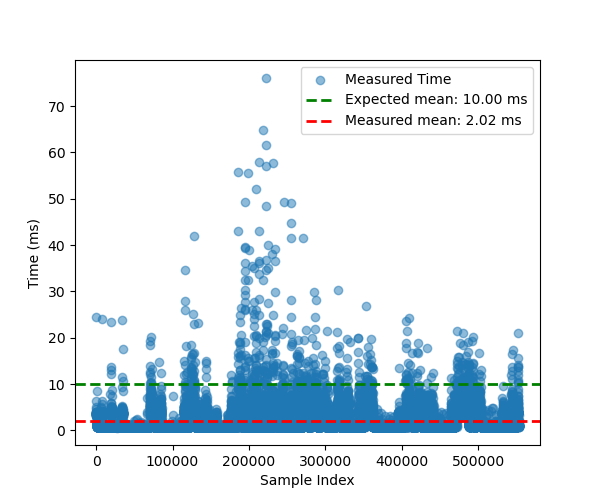
\includegraphics[width=1\linewidth]{figures/scatter_1000ssd_10ms.png}
    \caption{10ms event plot with 1ms SSD.} 
    \label{fig:1000ssd_10ms}
  \end{minipage}
  \hfill
  \begin{minipage}{0.5\textwidth}
    \centering
    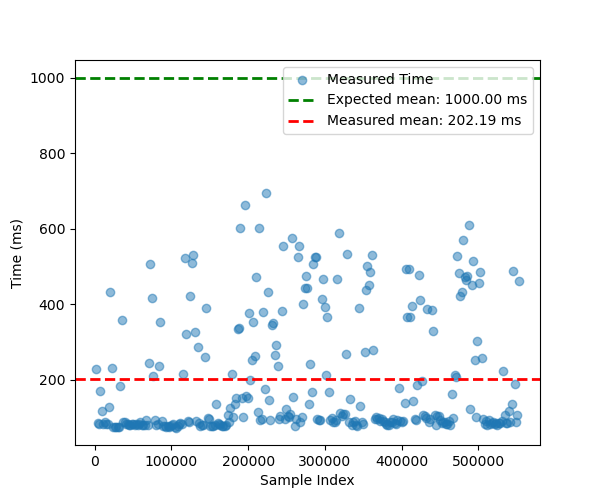
\includegraphics[width=1\linewidth]{figures/scatter_1000ssd_1s.png}
    \caption{1s event plot with 1ms SSD.} 
    \label{fig:1000ssd_1s}
  \end{minipage}
\end{figure}
From these plots, it became evident that there was a consistent deviation from real-time behavior. Specifically, the average time taken for each event was shorter than expected, suggesting an undesirable acceleration within the virtual environment. This deviation underscores the need for tighter synchronization between virtual and real-time execution to ensure accurate simulation results.

Interestingly, the timing deviation was consistent across different events, such as the 10ms and 100ms intervals. Upon further inspection of the SUTRunner's simulation code, we found that the system is driven by a timer interrupt managed by the "\textbf{ISR(Os\_TimerPfrtIsr)}" function, which is configured to trigger every 50 microseconds. Since all timing events are derived from this interrupt. This is why it`s expected that if one of the events goes slower the other events also go slower. When the SUTRunner was run with a simulation step duration of 1000 microseconds, the interrupt function was being called 20 times per simulation step, without any regard for real-time synchronization. This caused unadjusted virtual timing, making the simulation run faster than real time and preventing compensation for timing differences.


To address this, the initial solution involved reducing the simulation step duration to 50 microseconds, matching the interval of the interrupt function. This adjustment ensured that each simulation step directly aligned with the interrupt's timing. To account for the difference between virtual time and real time, we enabled a clock coupling thread on the SIL Kit. This thread checks after each simulation step if the virtual time is faster than the real time and waits until they equalize before proceeding to the next simulation step.

 \autoref{fig:50ssd_10ms} and \autoref{fig:50ssd_1s} show the results after implementing these modifications. Unfortunately, this approach did not yield the desired outcome. The events were slower than expected, likely due to the overhead associated with repeatedly calling the simulation function in very small time slices, as well as the additional tasks handled by the event loop. As a result, using 50-microsecond time slices proved ineffective for this architecture, leading to unsatisfactory performance.

\begin{figure}[h]
  \centering
  \begin{minipage}{0.49\textwidth}
    \centering
    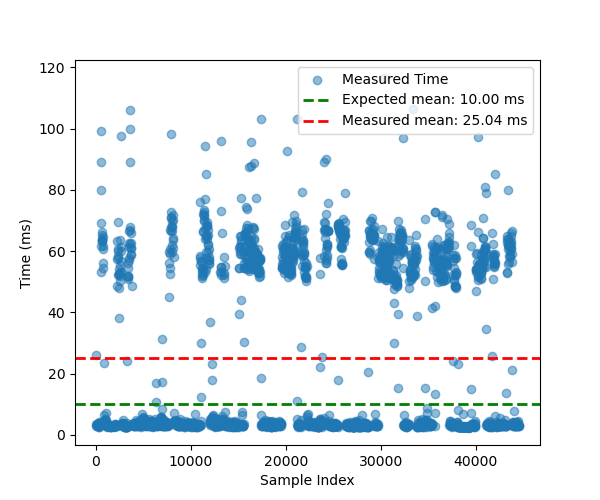
\includegraphics[width=1\linewidth]{figures/scatter_50ssd_10ms.png}
    \caption{10ms event Plot with 50$\mu$s SSD.} 
    \label{fig:50ssd_10ms}
  \end{minipage}
  \hfill
  \begin{minipage}{0.5\textwidth}
    \centering
    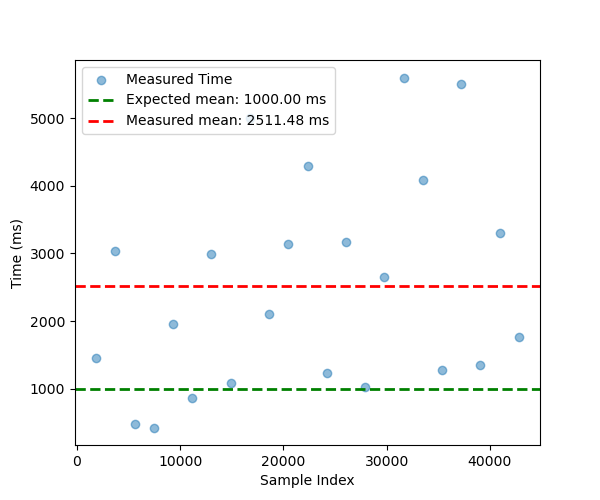
\includegraphics[width=1\linewidth]{figures/scatter_50ssd_1s.png}
    \caption{1s event Plot with 50$\mu$s SSD.} 
    \label{fig:50ssd_1s}
  \end{minipage}
\end{figure}

Considering that the smallest timing event in our simulation is 1ms, another strategy was to reconfigure the system by the timing of the interrupt function to be called every 1ms instead of 50 microseconds. This change would reduce the frequency of function calls and allow the simulation function to be called every 1000 microseconds, which is more aligned with the system's architecture. A clock coupling thread would still be necessary to maintain the balance between virtual and real time.

\autoref{fig:10ms_after}  and \autoref{fig:1s_after} show the results of this new approach for the 10ms and 1s events, respectively. The plots demonstrate that, after these adjustments, the virtual timing events now closely match real-time behavior. 

\begin{figure}[h]
  \centering
  \begin{minipage}{0.49\textwidth}
    \centering
    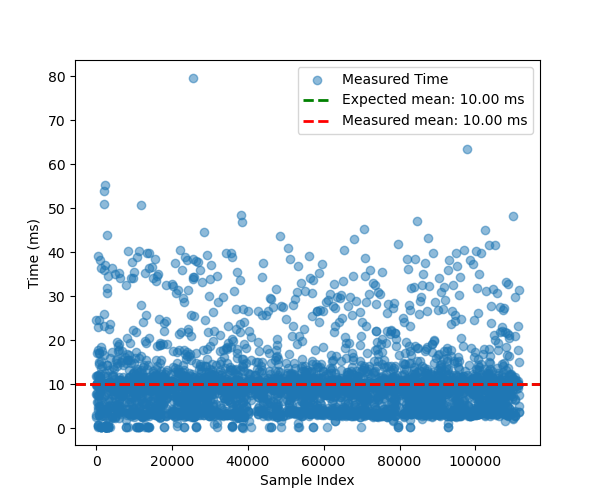
\includegraphics[width=1\linewidth]{figures/scatter_1000ssd_10ms_new.png}
    \caption{10ms event plot with 1ms SSD and 1ms timing interrupt.} 
    \label{fig:10ms_after}
  \end{minipage}
  \hfill
  \begin{minipage}{0.5\textwidth}
    \centering
    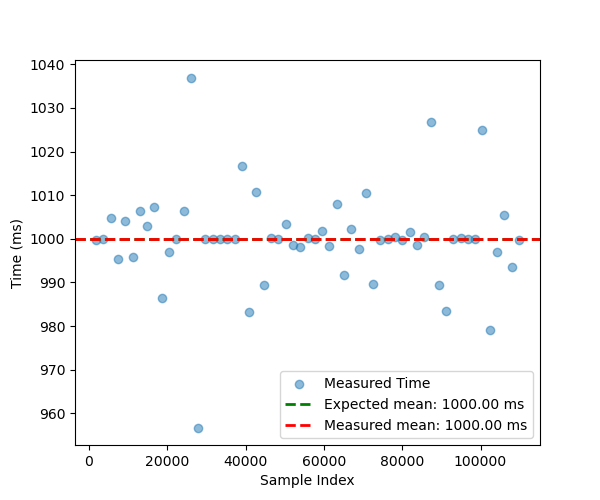
\includegraphics[width=1\linewidth]{figures/scatter_1000ssd_1s_new.png}
    \caption{1s event plot with 1ms SSD and 1ms timing interrupt.} 
    \label{fig:1s_after}
  \end{minipage}
\end{figure}


\begin{figure}[h]
  \centering
  \begin{minipage}{0.49\textwidth}
    \centering
    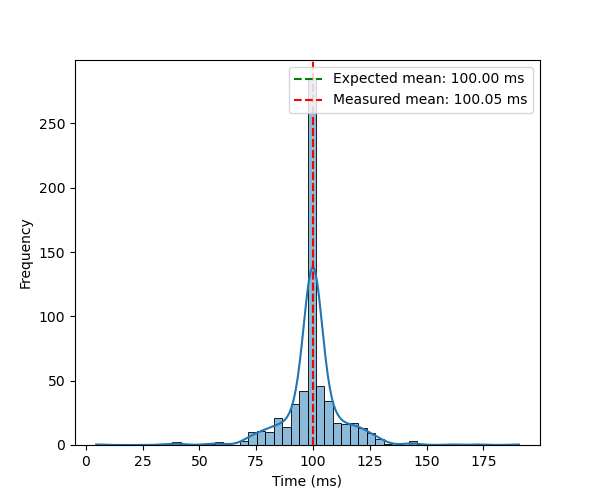
\includegraphics[width=1\linewidth]{figures/100ms_histogram_plot_new.png}
    \caption{100ms event histogram plot with 1ms SSD and 1ms timing interrupt.} 
    \label{fig:histogram_after}
  \end{minipage}
\end{figure}

\autoref{fig:histogram_after}  shows that the distribution of the 100ms timing event follows a normal distribution, with a mean of almost exactly 100ms, which is the expected and correct behavior.  These results confirm that, after implementing these modifications, the virtualized timing events now precisely align with the actual timing events on physical hardware, allowing for accurate and reliable simulation in the virtual environment.

\section{Correctness of the vECU}
To ensure the correctness of the virtual ECU (vECU), a series of real-world tests were conducted. These tests replicate the same procedures typically performed on a physical ECU, focusing on interactions between external components and the ECU, such as verifying the ability to install updates during the manufacturing process. The tests centered on sending Unified Diagnostic Services (UDS) requests from a testing tool to the vECU. 

To validate the vECU's response, a digital certificate was installed inside the vECU, and a series of UDS requests were sent to verify whether the system behaved as it would in a real ECU. A Python script was used to automate the process, sending the UDS requests and reading the certificate data from the vECU through UDS responses transmitted over the virtual CAN (vCAN) bus. The script was executed a hundred times to assess the robustness and consistency of the simulation. In each test iteration, the UDS requests were successfully delivered, and the vECU generated responses that matched the expected results, demonstrating the vECU’s correctness in handling diagnostic communication, just like a physical ECU would.

To demonstrate the virtual test environment's capability to execute a full set of tests for the BAC modules, four test suites, comprising 244 security-related tests, were run on both the virtual and hardware setups. The test suite contains robustness tests, this tests contain iterations of a feature, e.g. installing/deleting certificates 20 times. The tests executed in the virtual setup completed in 3 hours and 6 minutes, yielding identical results to those obtained on the hardware platform.

\section{Debugging}

A key objective of this project is not only to simulate the behavior of the ECU but also to enable a seamless debugging experience. Debugging in the virtual environment created for the vECU offers significant advantages over traditional real-time debugging on hardware.

In real-world testing with hardware, debugging usually involves connecting a hardware debugger to the ECU. This process is not only cumbersome but also limited by the hardware constraints. For example, real ECUs often have a finite number of hardware breakpoints—typically around eight. This limitation means that when debugging complex systems, the developer is restricted to setting a small number of breakpoints. Once the limit is reached, the debugger will refuse to set additional breakpoints, which can hinder the debugging process, especially when tracking down complex bugs that require observing multiple points in the code.

The virtualized environment for the vECU, however, overcomes these hardware constraints entirely. Using tools like GDB or the integrated debuggers in development environments, we can set an unlimited number of breakpoints in the virtual ECU without being restricted by hardware limitations. By being able to halt and inspect the execution at an infinite number of points, the virtual approach greatly enhances the debugging process, allowing more thorough and efficient issue resolution.